Let $\mathcal{H} = L^2 (0,1)$. We consider the stochastic Fisher-KPP 
    equation 
    \begin{equation}
        \label{eqn:fisher-kpp}
        \begin{aligned}
            d X(t, \xi) &= 
                \left[
                    \nu 
                    \partial_{\xi} ^ 2 X(t, \xi)
                    +
                    X(t, \xi) (1 -X(t, \xi) )
                \right]
                dt
                +
                dW(t, \xi),
            \\
            X(t, 0) &= X(t, 1) =0, \quad t>0, 
            \\
            X(0, \xi) & \in 
            \mathcal{H}, \ \xi \in [0, 1],
        \end{aligned}
    \end{equation}
    in the interval $[0, 1]$ and with initial function conditions
    $x(\xi))$ and  $\widehat{x}(\xi)$. In order to fix this initial function 
    conditions  close, we use for our experiments
    \begin{equation}
        x(\xi) := \sech ^ 2( 5  (\xi - 0.5)),
        \qquad
        \widehat{x}(\xi) :=
            \sum_{k=0} ^ N
             T_k(x(\xi)),
    \end{equation}
    where $T_k(\cdot)$ denotes the Chebyshev polynomial of the first kind. That 
    is, $\widehat{x}(\cdot)$ is the Chebyshev truncated expansion of $x(\cdot)$.
    
    \Cref{fig:fisher_kpp_approximation_t0} displays the 
    plots of this initial conditions. In \Cref{fig:likening_fisher_kpp} we 
    observe how the mentioned approximations remains close\textemdash blue
    color scale denotes the solution of equation \ref{eqn:fisher-kpp}
    with initial function condition $x(\xi)$, while yellow color corresponds 
    to the approximation with initial condition $\widehat{x}$. Since we employ
    transparency to obtain this 3D plot, the  purple scale results from the 
    closeness of the solutions. Further, \Cref{fig:errorfisher} suggest the 
    conclusion of \Cref{thm:ic_continuity}, that is, the solutions of equation
    \eqref{eqn:fisher-kpp} are continuous respect to initial conditions and 
    satisfies the estimation \eqref{s3.12}.

%
\begin{figure}[H]
    \centering
    \caption{
        Numerical Solution of the Fisher-KPP 
        \cref{eqn:fisher-kpp} 
        with initial conditions $x$, $\widehat{x}$ at time
        $t=0$.
     }
    \label{fig:fisher_kpp_approximation_t0}
    \includegraphics[width=\linewidth, keepaspectratio]%
    {StochasticFisherEquation/Approximation_t=0.eps}
\end{figure}
%
\begin{figure}[H]
    \centering
    \caption{
        Likening between two solution with closed 
        initial conditions $x$, $\widehat{x}$
        of the stochastic Fisher-KPP
        \cref{eqn:fisher-kpp}. See \cite{plotlyFisher}
        to obtain other camera perspectives.
     }
    \label{fig:likening_fisher_kpp}
    \includegraphics[width=\linewidth, keepaspectratio]%
    {StochasticFisherEquation/simulation_Approximation.png}
\end{figure}

%
%

\begin{figure}[htb]
    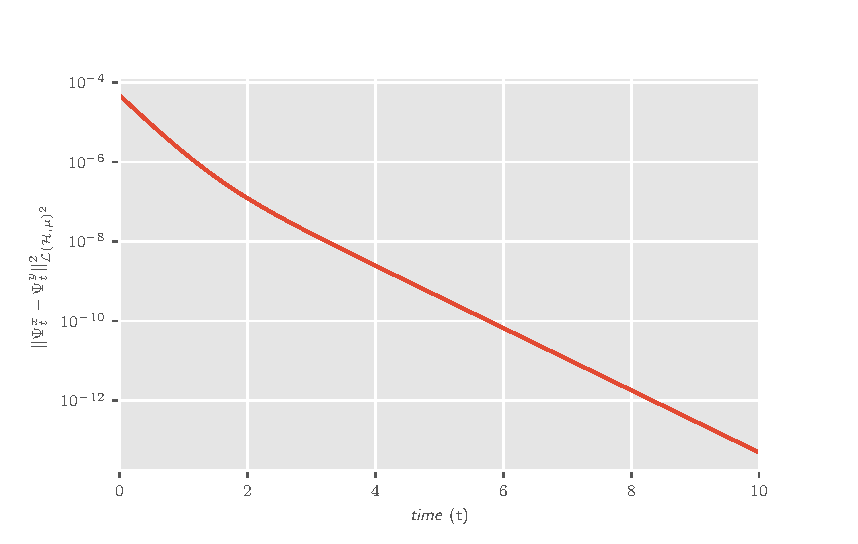
\includegraphics[width=\linewidth]{StochasticFisherEquation/error_fisher.eps}
    \caption{%
        $\mathcal{L}^2(\mathcal{H}, \mu)$
        distance between two solutions of the stochastic Fisher PDE 
        with initial conditions $x = x(\xi)$, and  $y = \widehat{x}(\xi)$.
    }
    \label{fig:errorfisher}
\end{figure}

    \Cref{fig:likening_fisher_kpp} illustrates the distance between initial 
conditions. The yellow pallet with transparency and a blue scale highlight the 
zones where the two solutions are close. Thus, the zones where the color is 
purple denotes, where the two solutions of SPDEs are close. 
According to the $\mathcal{L}( \mathcal{H}, \mu)$-distance between the two 
underlying solutions, \Cref{fig:errorfisher} confirms the above argument.

%